\section{LinkRank: A Learning-to-Rank Framework for O2M Issue--Commit Traceability}
% Brief: this section introduces our proposed LINKRANK framework for one-to-many issue--commit traceability, outlining its four main phases: dataset construction, feature representations, learning-to-rank model, and selection strategies.

% \subsection*{The \textsc{LinkRank} framework}

LinkRank is a learning-to-rank framework designed specifically for one-to-many issue--commit linking. Each issue acts as the query, and candidate commits are scored using a compact blend of lexical signals (TF--IDF + SVD) and retrieval focus (BM25), with ranking performed by a LambdaMART model. Selection proceeds via an \emph{iterative pick--remove--renormalize} loop that supports both Known-$K$ and Unknown-$K$ regimes, where $K$ denotes the true number of commits associated with an issue. We also study a complementary commit$\rightarrow$issue variant, \textit{LinkRank-C2I}, that performs bidirectional refinement. Our approach is organized into four phases. The complete workflow is illustrated in Figure~\ref{fig:approach}. 

% \begin{enumerate}
%     \setlength{\itemsep}{2pt}
%     \setlength{\parskip}{0pt}
%     \item Dataset construction
%     \item Feature representations
%     \item Learning-to-rank (LambdaMART)
%     \item Selection strategies
% \end{enumerate}

\begin{figure}[h!]
    \centering
    \includegraphics[width=\textwidth]{figures/App.png}
    \caption{Overall workflow of the proposed LINKRANK framework}
    \label{fig:approach}
\end{figure}

\subsection{Phase I: Dataset construction process}

% Brief: this subsection describes how repositories, issues, and commits were selected and filtered to build a one-to-many issue--commit dataset, and summarizes dataset statistics.

The dataset for this study was constructed using GitHub’s API to extract issue--commit pairs from multiple repositories. GitHub imposes a rate limit of 5,000 requests per hour per authenticated user, making data extraction a time-consuming process~\cite{GitHubAPI}. To ensure that the dataset captured realistic one-to-many relationships, we specifically filtered issues that were linked to at least two and at most six commits. Identifying repositories that contained a sufficiently large number of such issues proved challenging, as many projects either had too few one-to-many cases or exhibited extreme imbalance. Therefore, we selected repositories with a sufficient number of issues satisfying the 2–6 commit criterion. 

\begin{table*}[htbp]
\centering
\caption{Statistics of selected GitHub repositories used for dataset construction.}
% Reduce vertical density and horizontal padding so the table fits within page margins
\renewcommand{\arraystretch}{1.2}
\setlength{\tabcolsep}{4pt}
\label{stats}
\scriptsize
% Constrain the project name column to allow line-wrapping and avoid overflow
\begin{tabular}{p{2.5cm}ccccccc}
\hline
\multirow{2}{*}{\textbf{Project Name}} & 
\multirow{2}{*}{\textbf{Commits}} & 
\multirow{2}{*}{\textbf{Issues}} &
\multicolumn{5}{c}{\textbf{Number of Issues with N Commits}} \\ \cline{4-8}
 &  &  & \textbf{Two Commits} & \textbf{Three Commits} & \textbf{Four Commits} & \textbf{Five Commits} & \textbf{Six Commits} \\ \hline
Apache/Beam        & 3104 & 486 & 206 & 110 & 81 & 54 & 31 \\
Apache/Datafusion  & 3534 & 496 & 135 & 132 & 95 & 79 & 52 \\
Apache/Superset    & 3136 & 498 & 230 & 105 & 65 & 56 & 41 \\
Apache/Mxnet       & 1216 & 187 & 69 & 49 & 36 & 19 & 14 \\
Apache/Dubbo       & 1205 & 201 & 97 & 46 & 22 & 20 & 16 \\
Apache/Iceberg     & 1750 & 257 & 97 & 57 & 36 & 39 & 26 \\
Kubernetes         & 2948 & 483 & 238 & 102 & 66 & 43 & 31 \\
grpc               & 2162 & 486 & 131 & 84 & 51 & 34 & 28 \\
TensorFlow         & 2719 & 408 & 167 & 86 & 69 & 45 & 35 \\
PyTorch            & 748  & 125 & 51 & 45 & 14 & 9 & 6 \\ \hline
\end{tabular}
\end{table*}

The overall dataset statistics are summarized in Table~\ref{stats}, providing a detailed view of the scale and distribution of the collected data. This systematic filtering process ensured both the scalability of the dataset and its fidelity to real-world development practices.

\begin{table*}[htbp]
\centering
\caption{Programming languages in the selected GitHub repositories and their total stars.}
\label{tab:repo-langs}
\scriptsize
\renewcommand{\arraystretch}{1.3}
\setlength{\tabcolsep}{10pt}
\begin{tabular}{l l c c c c c c c}
\hline
	\textbf{Project} & \textbf{Owner} & \textbf{Stars} & \textbf{Java} & \textbf{Python} & \textbf{Rust} & \textbf{C++} & \textbf{Go} & \textbf{JS/TS} \\ \hline
Beam               & Apache     & 8.3k  & \ding{51} & \ding{51} & \ding{55} & \ding{55} & \ding{55} & \ding{55} \\
DataFusion         & Apache     & 7.7k  & \ding{55} & \ding{55} & \ding{51} & \ding{55} & \ding{55} & \ding{55} \\
Superset           & Apache     & 67.8k & \ding{55} & \ding{51} & \ding{55} & \ding{55} & \ding{55} & \ding{51} \\
MXNet              & Apache     & 20.8k & \ding{55} & \ding{51} & \ding{55} & \ding{51} & \ding{55} & \ding{55} \\
Dubbo              & Apache     & 41.3k & \ding{51} & \ding{55} & \ding{55} & \ding{55} & \ding{55} & \ding{55} \\
Iceberg            & Apache     & 7.9k  & \ding{51} & \ding{55} & \ding{55} & \ding{55} & \ding{55} & \ding{55} \\
Kubernetes         & Kubernetes & 117k  & \ding{55} & \ding{55} & \ding{55} & \ding{55} & \ding{51} & \ding{55} \\
gRPC (grpc)        & grpc       & 43.6k & \ding{55} & \ding{55} & \ding{55} & \ding{55} & \ding{51} & \ding{55} \\
TensorFlow         & TensorFlow & 191k  & \ding{55} & \ding{51} & \ding{55} & \ding{51} & \ding{55} & \ding{55} \\
PyTorch            & PyTorch    & 93.2k & \ding{55} & \ding{51} & \ding{55} & \ding{51} & \ding{55} & \ding{55} \\ \hline
\end{tabular}

\vspace{3pt}
\footnotesize{
    \ding{51} = present / primary language \quad\quad \ding{55} = not present / minor traces}
\end{table*}

Table~\ref{tab:repo-langs} summarizes the primary programming languages used in each selected repository, highlighting the diversity of languages (Java, Python, Rust, C++, Go, JavaScript/TypeScript) represented in our dataset. This variety ensures that our approach is evaluated across different coding styles and practices, enhancing its generalizability. The languages were identified using GitHub's Linguist tool, which analyzes the repository contents to determine the primary programming languages used.


\subsubsection*{False Link Generation}

% Brief: this subsubsection explains our PR-aware strategy for creating realistic negative samples (false links) that balance positives per-issue while avoiding semantic overlap.

Constructing a reliable set of false links is critical for evaluating issue-commit link recovery models, as it enables a more accurate assessment of the models' ability to distinguish between correctly linked and mismatched issue-commit pairs. However, previous works have often faced challenges in generating false links, which may compromise the quality of the datasets used for model evaluation. Thus, we propose a novel approach for generating false links that addresses these challenges.\\

\noindent
Several existing studies have relied on simplistic strategies for generating false links, which can lead to inaccuracies. For example, BTLink \cite{btlink} and DeepLink \cite{q1} generated false links by randomly pairing issues and commits from separate projects or unrelated time periods. This approach risks introducing semantically related links that were mistakenly labeled as false, as code changes made in close time proximity or in related repositories may still be connected to the same issue. Similarly, HERMES \cite{hermes} and EALink \cite{ealink} created false links using time-based sampling techniques, where issues and commits were paired if they were not linked within a specific time frame. However, this method overlooks the possibility that complex issue resolutions may involve multiple commits spread over extended periods, potentially leading to the inclusion of valid links being mislabeled as false. Additionally, T-BERT \cite{tbert} generated a large number of false links without verifying their semantic separation from true links, leading to datasets where negative pairs may still be contextually relevant, thus reducing the reliability of the ground truth.\\


% \begin{figure*}[htbp] % t=top, b=bottom, h=here, H=exact (needs \usepackage{float})
%   \centering
%   \includegraphics[width=\linewidth]{qwqwqwqwq.png}
%   \caption{Overall workflow of the proposed \textsc{LinkRank} framework, illustrating its four main phases: Data preparation, Feature Representations, Learning-to-Rank, and Selection Strategies.}
%   \label{approach}
% \end{figure*}



% \begin{figure*}[t] % t=top, b=bottom, h=here, H=exact (needs \usepackage{float})
%   \centering
%   \includegraphics[width=\linewidth]{App.png}
%   \caption{Overall workflow of the proposed \textsc{LinkRank} framework, illustrating its four main phases: Data preparation, Feature Representations, Learning-to-Rank, and Selection Strategies.}
%   \label{approach}
% \end{figure*}

To address these limitations, we adopt a Pull Request (PR)-aware strategy for generating false links. We first identify valid PRs that satisfy our condition of having between 2 and 6 commits. For each valid PR $p$, we denote its corresponding issue as $i_p$ and the set of associated commits as $C_p = \{c_1, c_2, \dots, c_m\}$, where $2 \leq m \leq 6$. The set of true links is therefore defined as $T = \{(i_p, c_j) \mid p \in \mathcal{P}_{\text{valid}},\; c_j \in C_p\}$.\\

Next, we consider PRs that do not satisfy the 2--6 commit constraint, denoted as $\mathcal{P}_{\text{invalid}}$. From these PRs, we construct a pool of unrelated commits:
\[
C_{\text{invalid}} = \bigcup_{p \in \mathcal{P}_{\text{invalid}}} C_p.
\]

For each valid issue $i_p$ with $m = |C_p|$ true commits, we generate an equal number of false links by randomly sampling $m$ unrelated commits from $C_{\text{invalid}}$. This ensures that the number of false links matches the number of true links on a per-issue basis: $F_p = \{(i_p, c_r) \mid c_r \sim \text{Uniform}(C_{\text{invalid}}), \; |F_p| = m \}$.\\

\noindent
Finally, the dataset is formed by combining true and false links, i.e., $D = T \cup \bigcup_{p \in \mathcal{P}_{\text{valid}}} F_p$.\\

\noindent
This construction guarantees balance between positive and negative samples for each issue, while keeping the false links realistic and repository-aware. The PR-aware false link generation strategy minimizes the risk of semantic overlap between true and false links, thereby enhancing the reliability of the dataset for evaluating issue-commit link recovery models.


\subsection{Phase II: Feature Representations}

% Brief: this subsection describes the feature channels (lexical, retrieval-based, semantic) used to encode issue--commit pairs into compact vectors for ranking.

To effectively model the one-to-many issue--commit linking problem, each candidate pair $(i,c)$ is encoded into a feature vector $x_{ic}$ that captures complementary dimensions of similarity. Rather than relying on a single view of the data, we combine lexical, retrieval-based, and optional semantic features, enabling the model to distinguish true links from superficially similar but incorrect ones. 

\subsubsection{Lexical Similarity (TF--IDF + SVD).}
% Brief: explains the TF--IDF + truncated SVD lexical channel and the cosine similarity feature used to quantify lexical alignment between issues and commits.
For the lexical perspective, we employ Term Frequency--Inverse Document Frequency (TF--IDF), a well-established method in information retrieval for quantifying the salience of terms relative to a corpus. The TF component reflects how often a term appears in a document (issue or commit), while the IDF component down-weights terms that are frequent across the whole corpus and up-weights rarer, more discriminative terms. To capture latent topics and reduce dimensionality, we apply truncated Singular Value Decomposition (SVD), yielding compact dense representations. The cosine similarity between an issue vector $v_i$ and a commit vector $v_c$ is then
\[
f_{\text{text}}(i,c) = \frac{\langle v_i, v_c \rangle}{\|v_i\|\cdot \|v_c\|},
\]
where $\langle v_i, v_c \rangle$ is the dot product and $\|v_i\|$, $\|v_c\|$ are vector norms. High values indicate strong lexical alignment, while the SVD projection smooths sparsity and captures latent semantics beyond exact token overlap.

\subsubsection{BM25 Matching.}
% Brief: describes BM25 as a query-focused retrieval score that models term importance and document length for issue-as-query vs. commit-as-document matching.
While TF--IDF provides global representations, retrieval often benefits from query-focused matching. BM25 \cite{bm25}, a probabilistic ranking function widely used in search engines, is particularly effective here. It improves upon TF--IDF by modeling diminishing returns for repeated term occurrences and by normalizing document length, thus avoiding bias toward longer commit messages. Treating the issue text as a query and the commit text as a document, BM25 yields
\[
f_{\text{bm25}}(i,c) = \sum_{t \in i} \text{IDF}(t) \cdot 
\frac{f(t,c)\cdot (k_1+1)}{f(t,c) + k_1\!\cdot\!\left(1 - b + b \cdot \tfrac{|c|}{\text{avgdl}}\right)}.
\]
Here, $\text{IDF}(t)$ emphasizes rare terms, $f(t,c)$ counts term occurrences in commit $c$, $|c|$ is the commit length, $\text{avgdl}$ is the average commit length in the \emph{training} corpus, $k_1$ controls frequency saturation, and $b$ tunes length normalization. In this way, BM25 captures how well a commit matches an issue when the issue is interpreted as a retrieval query.



\subsubsection{Semantic Similarity (CodeBERT).}
% Brief: outlines the optional CodeBERT-based semantic channel which provides vector embeddings to capture paraphrases and code-aware context beyond lexical signals.
In addition to lexical and retrieval features, we include a complementary semantic signal from CodeBERT \cite{codebert}, a transformer model pre-trained on natural language and code. We compute mean-pooled embeddings $\phi(i)$ and $\phi(c)$ for the issue and commit, L2-normalize them, and score with cosine similarity:
\[
f_{\text{sem}}(i,c) = \cos\big(\phi(i), \phi(c)\big).
\]
This semantic channel complements TF--IDF and BM25 by capturing paraphrases and code-aware context (e.g., terse messages or alternate phrasings). Importantly, our ablations show that the model remains strong \emph{without} CodeBERT; adding it primarily improves robustness in cases where wording diverges or context is sparse.






\subsection{Phase III: Learning-to-Rank with LambdaMART}
% Brief: describes training a LambdaMART ranker on the extracted feature vectors (grouped by issue) to directly optimize ranking metrics for one-to-many recovery.
To transform the extracted feature representations into an effective linking model, we employ \textit{LambdaMART} \cite{lambda}, a gradient boosted decision tree algorithm specifically designed for ranking tasks. Unlike conventional classification methods that predict binary labels, LambdaMART directly optimizes ranking-based metrics such as the Normalized Discounted Cumulative Gain (NDCG), making it particularly well suited for the one-to-many issue--commit linking problem.


The central idea is to model relative preferences between commits for each issue. Training data are grouped by issue, ensuring that the model does not learn absolute scores across unrelated issues, but instead learns how to order candidate commits within each issue context (Algorithm~\ref{algo_1}). Given the feature vector $x_{ic}$ for an issue--commit pair $(i,c)$, LambdaMART learns a non-linear scoring function $\mathcal{R}$ through gradient-boosted regression trees. The output of the model is a ranking score:
\[
s(i,c) = \mathcal{R}(x_{ic}),
\]
where higher scores indicate stronger likelihood of a true issue--commit link.

This formulation offers two key benefits. First, it allows the model to focus directly on ranking quality rather than classification accuracy, which is crucial in settings where each issue may be linked to multiple commits. Second, tree-based boosting naturally captures complex, non-linear feature interactions (e.g., when lexical similarity is high but BM25 matching is weak, or when semantic similarity diverges), yielding a more discriminative and flexible ranking function. At inference time, we score a pool of candidate commits for each issue and then apply an \emph{iterative} selection rule: we pick the current top commit, remove it from the pool, recompute per-issue normalization $\tilde{s}(i,c)$ (min--max scaled) and the updated $s_{\max}$, and repeat until the stopping rule is met. Thus, LambdaMART forms the foundation of our \textsc{LinkRank} framework, enabling robust recovery of one-to-many issue--commit links.


\subsection{Phase IV: Selection Strategies}
% Brief: explains iterative post-processing policies (Known-K oracle and two Unknown-K thresholding rules) that convert per-issue rankings into final one-to-many link sets.
Once the ranking scores are obtained, the final prediction set $\widehat{\mathcal{C}}(i)$ for each issue $i$ must be constructed. We follow an \emph{iterative pick--remove--renormalize} procedure: at each step, select according to the chosen policy, remove the selected commit from the pool, and recompute per-issue normalization (min--max $\tilde{s}$) and the current $s_{\max}$ before the next step. We distinguish between two cases:  

\paragraph{Known-K} In this case, we assume that the true number of commits $K$ associated with issue $i$ is known (an oracle setting). We iteratively take the top-ranked commit, remove it, renormalize scores, and continue until exactly $K$ commits have been selected. Although impractical in deployment (since the true $K$ is rarely available), this strategy serves as an important upper bound to evaluate the performance of our framework. 

\paragraph{Unknown-K} In this case, the number of commits linked to each issue is not known beforehand. This makes the task considerably harder, as the system must automatically determine not only which commits to link, but also how many. To address this challenge, we introduce two threshold-based strategies that adapt selection to the relative or absolute quality of ranking scores:
\begin{itemize}
    \item \textit{Absolute Thresholding (ABS):} At each iteration, after renormalization, link any commit whose normalized score $\tilde{s}(i,c)$ exceeds a fixed threshold $\tau$; remove selected commits and repeat until no remaining candidate exceeds $\tau$. This imposes a global cutoff across issues.
    \item \textit{Relative Thresholding (REL):} At each iteration, with the current top score $s_{\max}(i)$, link any commit satisfying $s(i,c) \ge \gamma \cdot s_{\max}(i)$; remove selected commits, recompute $s_{\max}(i)$, and continue until no remaining candidate satisfies the $\gamma$ criterion. This adapts to per-issue score scales.
\end{itemize}

Together, these strategies allow us to contrast oracle-based performance (Known-K) with more realistic scenarios (Unknown-K). The ABS rule emphasizes global calibration, while the REL rule emphasizes local adaptivity, and both operate within the same iterative pick--remove--renormalize loop, making them well-suited for the one-to-many linking problem.



\begin{algorithm}[htbp]
\caption{LinkRank }
\label{algo_1}
\begin{algorithmic}[1]
\STATE \textbf{Input:} Issues $\mathcal{I}$, commits $\mathcal{C}$, labeled pairs $\mathcal{D}$
\STATE \textbf{Output:} Predicted links $\{\widehat{\mathcal{C}}(i)\}_{i\in\mathcal{I}}$
\STATE Build corpora $S_{\mathcal{I}}, S_{\mathcal{C}}$; compute TF--IDF{+}SVD and BM25 features; \textit{(optional) }CodeBERT features
\FORALL{$(i,c,y)\in\mathcal{D}$}
  \STATE Build feature $x_{i,c}$ 
\ENDFOR
\STATE Train LambdaMART ranker $\mathcal{R}$ grouping by \textbf{Issue ID}
\FORALL{$i\in\mathcal{I}$}
  \FORALL{$c\in\mathcal{C}$}
    \STATE $s(i,c)\gets \mathcal{R}(x_{i,c})$
  \ENDFOR
  \STATE Compute per-issue normalized scores $\tilde{s}(i,c)$ via min--max; let $s_{\max}(i)\gets \max_{c}s(i,c)$
  \STATE \textit{Iterative selection:} repeat
  \STATE \hspace{0.6cm}Pick $c^\star \in \arg\max_{c} s(i,c)$ if admissible by the chosen policy
  \STATE \hspace{0.6cm}Add $c^\star$ to $\widehat{\mathcal{C}}(i)$; remove $c^\star$ from the candidate pool
  \STATE \hspace{0.6cm}Recompute $\tilde{s}(i,c)$ (min--max) and update $s_{\max}(i)$
  \STATE until stopping criterion is met
  \STATE \textbf{Selection policies:}
  \STATE \hspace{0.6cm}\textbf{Known-$K$:} select exactly the top $K$ commits
  \STATE \hspace{0.6cm}\textbf{Unknown-$K$ (ABS):} select all $c$ with $\tilde{s}(i,c)\ge \tau$
  \STATE \hspace{0.6cm}\textbf{Unknown-$K$ (REL):} select all $c$ with $s(i,c)\ge \gamma \cdot s_{\max}(i)$
\ENDFOR
\end{algorithmic}
\end{algorithm}


\subsection{Phase V: Bidirectional Variant: LinkRank-C2I}

In addition to our primary framework, \textsc{LinkRank}, which adopts an issue-centric perspective, we also experimented with a variant called \textsc{LinkRank-C2I} (commit$\rightarrow$issue). The motivation is to provide a complementary view by reversing the linking perspective. Since issue--commit relationships are inherently bidirectional, examining the task from the commit side lets us study whether different linking dynamics emerge when commits are treated as queries, and it further enables a consistency check between both directions, as detailed in Algorithm~\ref{algo_2}.\\

\noindent
\textbf{Step 1: Commit-to-Issue Retrieval.}\ \
Each commit $c \in \mathcal{C}$ is treated as a query and issues $i \in \mathcal{I}$ are candidates. Feature representations (TF--IDF+SVD, BM25, and optional CodeBERT) are computed exactly as in \textsc{LinkRank}, but tuples are grouped by \textbf{commit} for training. A LambdaMART ranker $\mathcal{R}_{A2}$ learns to score candidate issues:
\[
s_{A2}(c,i) = \mathcal{R}_{A2}(x_{c,i}),
\]
where $x_{c,i}$ is the feature vector for commit $c$ and issue $i$. To restrict the search space, we retain only the top-$K$ issues per commit:
\[
\mathcal{S}(c) = \mathrm{Top}\text{-}K \{\, i \in \mathcal{I} \mid s_{A2}(c,i) \,\}.
\]
(Optionally, a BM25 guard can expand the candidate set with a few high-recall issues per commit.)

\noindent
\textbf{Step 2: Issue-to-Commit Validation.}\ \
We then reintroduce the issue-centric view of \textsc{LinkRank}. For each issue $i$, we restrict its candidate pool to those commits that shortlisted $i$ in Step~1:
\[
\mathcal{P}(i) = \{\, c \in \mathcal{C} \mid i \in \mathcal{S}(c) \,\}.
\]
The Issue-to-Commit ranker $\mathcal{R}_{A1}$ (trained by grouping tuples \textbf{by issue}) is applied to this reduced pool, producing refined scores:
\[
s(i,c) = \mathcal{R}_{A1}(x_{i,c}), \quad c \in \mathcal{P}(i).
\]
This cross-directional gating enforces agreement between the commit$\rightarrow$issue and issue$\rightarrow$commit views.\\

% typically reducing false positives while preserving recall.



\begin{algorithm}[htbp]
\caption{LinkRank-C2I}
\label{algo_2}
\begin{algorithmic}[1]
\STATE \textbf{Input:} Issues $\mathcal{I}$, commits $\mathcal{C}$, labeled pairs $\mathcal{D}$
\STATE \textbf{Output:} Predicted links $\{\widehat{\mathcal{C}}(i)\}_{i\in\mathcal{I}}$
\STATE Build corpora $S_{\mathcal{I}}, S_{\mathcal{C}}$; compute TF--IDF{+}SVD and BM25 features; \textit{(optional) }CodeBERT features
\FORALL{$(i,c,y)\in\mathcal{D}$}
  \STATE Build feature $x_{i,c}$ 
\ENDFOR
\STATE Train commit$\rightarrow$issue ranker $\mathcal{R}_{\text{C2I}}$ (group by \textbf{Commit ID}) and issue$\rightarrow$commit ranker $\mathcal{R}_{\text{I2C}}$ (group by \textbf{Issue ID})

\vspace{0.25em}
\STATE \textbf{Stage 1 ,  Commit$\rightarrow$Issues (shortlist)}
\FORALL{$c\in\mathcal{C}$}
  \STATE $s_{\text{C2I}}(c,i)\gets \mathcal{R}_{\text{C2I}}(x_{c,i})$ for all $i\in\mathcal{I}$
  \STATE shortlist $\mathcal{S}(c)\gets$ top-$K$ issues ranked by $s_{\text{C2I}}$
\ENDFOR

\vspace{0.25em}
\STATE \textbf{Stage 2 ,  Issue$\rightarrow$Commits (final selection)}
\FORALL{$i\in\mathcal{I}$}
  \STATE pool $\mathcal{P}(i)\gets \{\,c\in\mathcal{C}: i\in\mathcal{S}(c)\,\}$
  \STATE $s(i,c)\gets \mathcal{R}_{\text{I2C}}(x_{i,c})$ for $c\in\mathcal{P}(i)$
  \STATE sort by $s$; let $s_{\max}$ be top; compute per-issue $\tilde{s}$ (min--max)
  \STATE \textit{Iterative rule}: after each pick, remove it from $\mathcal{P}(i)$ and recompute per-issue normalization
  \STATE \textbf{Selection strategies:} apply Known-$K$, Unknown-$K$ ABS, or Unknown-$K$ REL as in Algorithm~\ref{algo_1}
\ENDFOR
\end{algorithmic}
\end{algorithm}

\noindent
\textbf{Selection Strategies.}\ \
We use the same policies as in \textsc{LinkRank} (Known-$K$, Unknown-$K$ ABS, and Unknown-$K$ REL) with the same \emph{iterative} procedure: pick the current best commit for $i$, remove it from $\mathcal{P}(i)$, recompute per-issue normalization (min--max $\tilde{s}$) and the updated $s_{\max}(i)$, and continue until the stopping rule is met. In summary, \textsc{LinkRank-C2I} complements the primary approach by enforcing bidirectional consistency, typically reducing false positives while preserving recall.


